\documentclass[10pt]{beamer}

%STANDARD PREAMBLE
%https://tex.stackexchange.com/questions/68821/is-it-possible-to-create-a-latex-preamble-header
%\usepackage{/Users/mwojno01/Repos/latex_preamble/beamer_preamble}
\usepackage{/Users/miw267/Repos/csci246_spring2025/slides/preambles/beamer_preamble_for_CSCI246}


%%%
% SPECIFIC TO THIS DOCUMENT 
%%%
\let\warning\relax
\usepackage{fourier} % has warning  and danger symbols. However, it makes the bottoms tuff bold. 

\renewcommand{\ELBO}{\texttt{ELBO}}
\renewcommand{\Q}{\mathcal{Q}}


%%%%
% DOCUMENT 
%%%
\title{03/12/2026: Variational Autoencoders}
\author{Reference: \textit{Autoencoding Variational Bayes}}
\date{CSCI 546: Diffusion Models}

\begin{document}
\maketitle

%\begin{frame}{Table of contents}
%  \setbeamertemplate{section in toc}[sections numbered]
%  \tableofcontents[hideallsubsections]
%\end{frame}

\begin{frame}{Table of contents}
  \setbeamertemplate{section in toc}[sections numbered]
  \setbeamertemplate{subsection in toc}[subsections numbered]
  \tableofcontents
\end{frame}

\section{Course Logistics}


\begin{frame}
\begin{center}

\includegraphics[width=.6\textwidth]{images/DataFest 2026 blue.pdf}	
\end{center}
\end{frame}



\begin{frame}
\begin{myredbox}[title=Lightning Chats]
\begin{itemize}
	\item After Spring Break, any class meeting associated with a reading will have one $\approx$ 10 minute peer \textbf{lightning chat}.  
	\item The lightning chats will be given by groups of two. I will do the best I can to assign groups based on your preferences. 
	\item Sometime \textbf{today}, please either hand me or email me a list of three readings that are particular interest to you.  You can order them if you want.  You can name people you'd like to work with. 
	\item If I don't get your preferences today, I will randomly assign you to a partner and paper.
\end{itemize}
\end{myredbox}
\end{frame}


\begin{frame}{Reading Survey}

\begin{enumerate}
	\item What is a \underline{variational} autoencoder?
\end{enumerate}
	
\end{frame}

\section{Overview of VAEs}

\begin{frame}{Goal}

\begin{center}
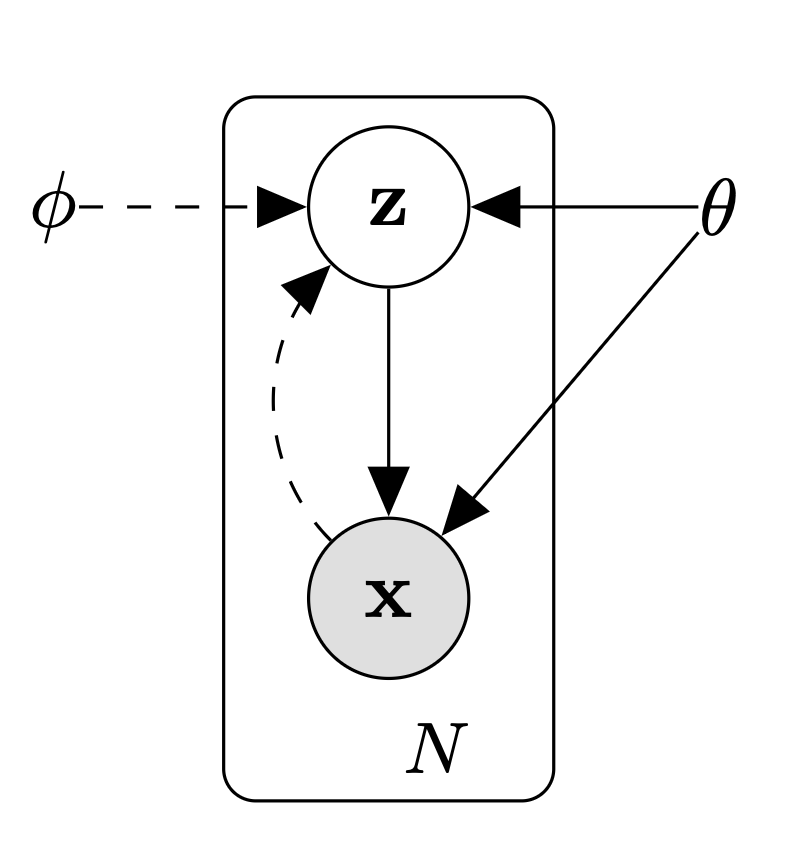
\includegraphics[width=.4\textwidth]{images/vae_high_level.png}
\end{center}

\colorbox{green!30}{\textbf{Goal.}} Learn a probabilistic model giving a low-dimensional latent variable ($\+z$) representation of the data ($\+x$) distribution, \pause which allows:
\begin{itemize}
	\item \textit{Reconstruction}:  Can the model reproduce something it has seen? \pause 
	\item \textit{Generation}: Can the model create new examples that look like the dataset?
\end{itemize}

	
\end{frame}

\begin{frame}{Comparison to previous approaches}
\small 
\only<1->{
We want the latent ''code'' to 
\begin{enumerate}
	\item Capture \alert{nonlinear structure} in the data, going beyond linear dimensionality reduction methods like principal component analysis, and 
	\item Support \alert{probabilistic generative model} of the data. \only<2->{This allows us to sample new data, and also gives well-structured latent space.}
\end{enumerate}
}



\only<3>{
\begin{figure}
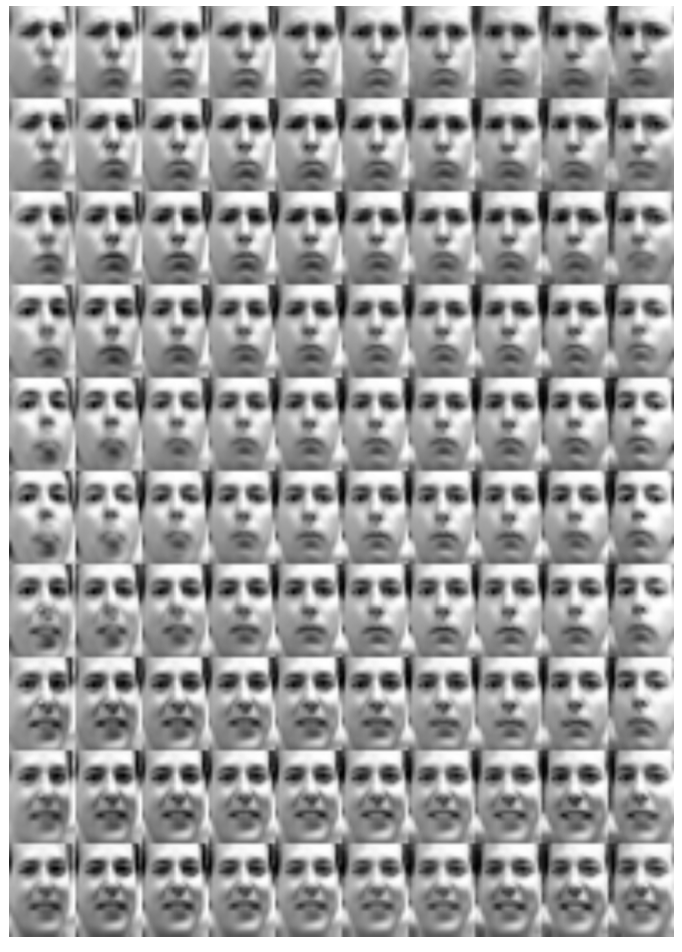
\includegraphics[width=.35\textwidth]{images/learned_frey_face_manifold}
%\caption{Learned Frey Face Manifold}
\end{figure}
}

\only<4>{
\begin{figure}
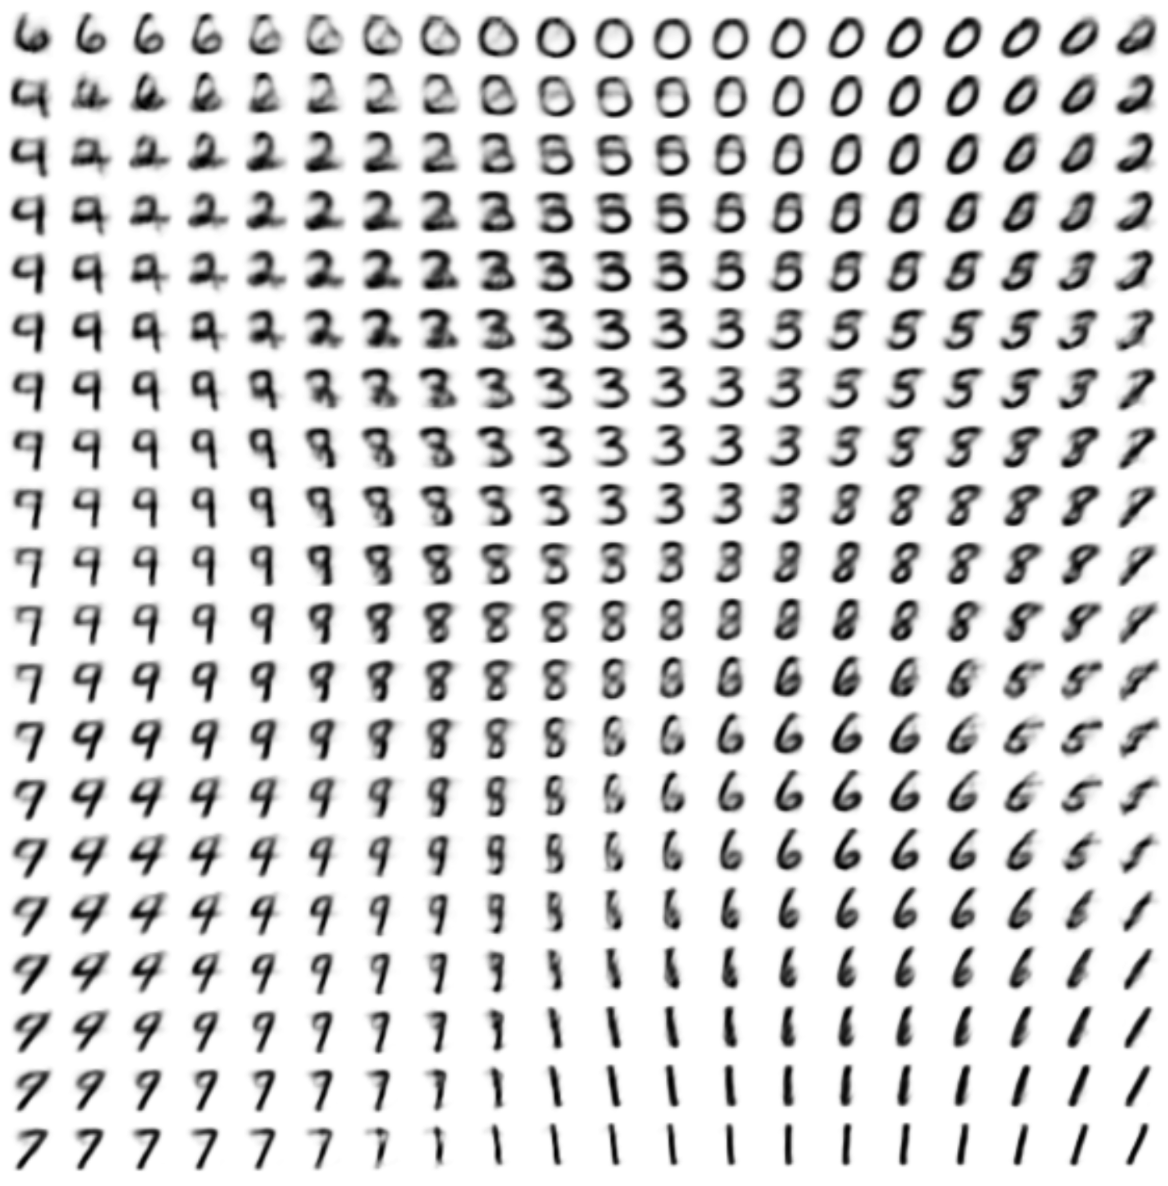
\includegraphics[width=.45\textwidth]{images/learned_MNIST_manifold}
%\caption{Learned MNIST Manifold}
\end{figure}
}
	
	
\end{frame}


\begin{frame}{How to construct  a flexible probabilistic encoder/decoder?}

\pause 
\colorbox{green!30}{\textbf{Idea.}} Parameterize  Conditional Distributions with Neural Networks!

\vfill 


\begin{center}
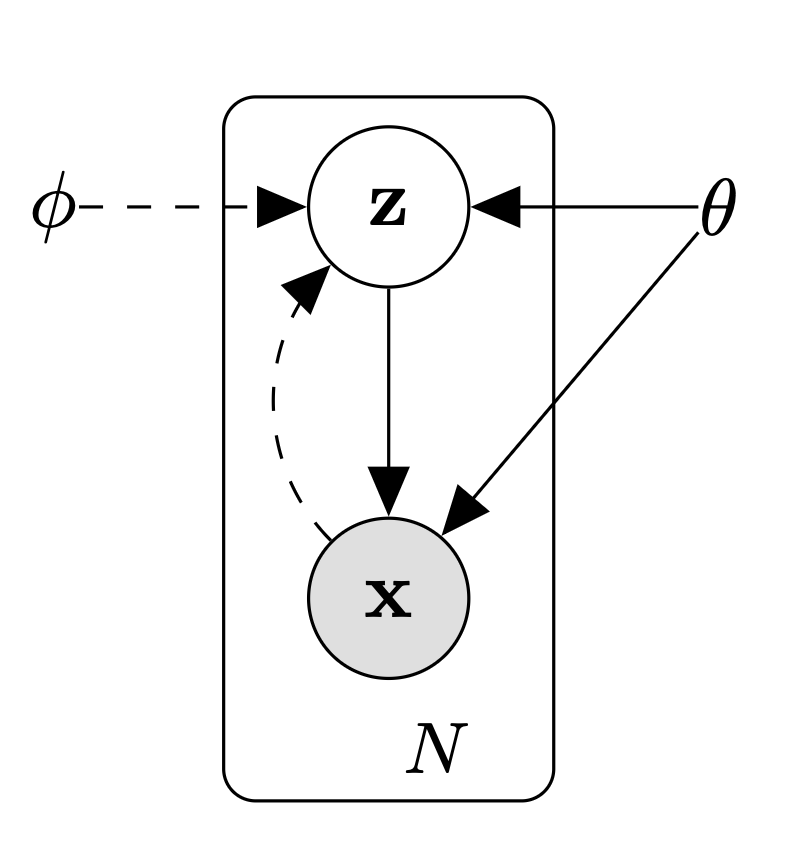
\includegraphics[width=.4\textwidth]{images/vae_high_level.png}
\end{center}

\pause 

\begin{minipage}{0.48\textwidth}
\centering
\textbf{Encoder}

\begin{align*}
(\+\mu_\+x, \log \+\sigma_\+x) &= \texttt{NeuralNetwork}_\phi (\+x) \\
 q_\phi(\+z \mid \+x) &= \N \big(\+z ; \+\mu_\+x, \text{diag} (\+\sigma^2_\+x) \big)
\end{align*}

\end{minipage}
\hfill
\begin{minipage}{0.48\textwidth}
\centering
\textbf{Decoder}

\begin{align*}
(\+\mu_\+z, \log \+\sigma_\+z) &= \texttt{NeuralNetwork}_\theta (\+z) \\
 p_\theta(\+x \mid \+z) &= \N \big(\+x ; \+\mu_\+z, \text{diag} (\+\sigma^2_\+z) \big)
\end{align*}

\end{minipage}

	
\end{frame}


\begin{frame}{Bayesian Perspective}
\small 

\begin{center}
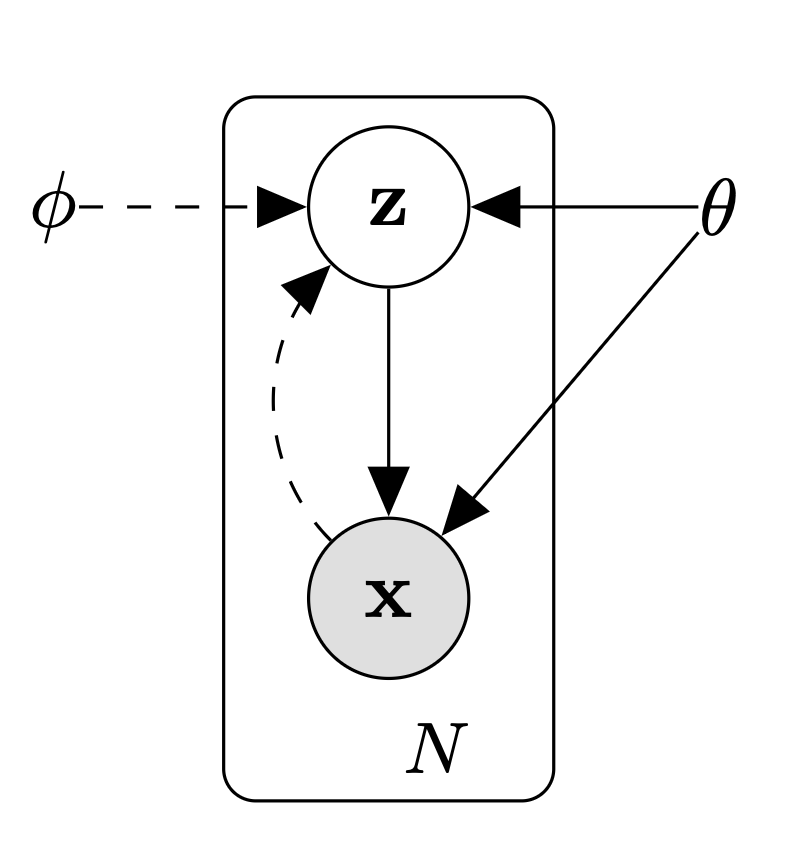
\includegraphics[width=.3\textwidth]{images/vae_high_level.png}
\end{center}

\begin{align*}
 p(\+z) &= \N \big(\+z ; \+0, \+I \big) && \textbf{Prior} \\  
 p_\theta(\+x \mid \+z) &= \N \big(\+x ; \+\mu_\+z, \text{diag} (\+\sigma^2_\+z) \big) && \textbf{Likelihood}  \\
  q_\phi(\+z \mid \+x) &= \N \big(\+z ; \+\mu_\+x, \text{diag} (\+\sigma^2_\+x) \big) && \textbf{(Variational) Posterior}
\end{align*}

\pause 

\colorbox{blue!30}{\textbf{Remark.}}  The prior here is serving a different purpose than classical Bayesian models.
\begin{itemize}
\item In \textbf{classical Bayes}, the prior expresses knowledge about the world.
\item In a \textbf{VAE}, the prior expresses how we want the latent space to be organized.
\end{itemize}

\end{frame}


\begin{frame}{Gaussian latent variable models}
	

\only<2->{
We can interpret a VAE as a \alert{\texttt{nonlinear}} Gaussian latent variable model.
}

\only<3>{
\vfill 
\begin{mybluebox}[title=\text{Classical \texttt{linear} Gaussian latent variable model}] In models like probabilistic Principal Components Analysis (PCA):

\begin{align*}
\+z & \sim \mathcal N(\+0,\+I)	 \\
\+x \mid \+z &\sim \mathcal N(\+W\+z + \+b,; \sigma^2 \+I)
\end{align*}
 
Key properties:

\begin{itemize}
	\item Latent variable ($\+z$) is Gaussian
	\item Observation ($\+x$) is Gaussian with a mean that is a \alert{linear function} of $\+z$:
	\[ \+\mu_\+z = \+W\+z + \+b \]
\end{itemize}

%So the model is a Gaussian latent variable model with \alert{linear} mean structure.
\end{mybluebox}

}



\only<4>{
\vfill 
\begin{mybluebox}[title=\text{VAE as a \texttt{nonlinear} Gaussian model}.] 
	

In a VAE:

\begin{align*}
\+z & \sim \mathcal N(\+0,\+I)	 \\
\+x \mid \+z &\sim \mathcal N\big(f_\theta(\+z), \text{diag}(g_\theta(\+z))\big)
\end{align*}
% 
where now $f_\theta$ and $g_\theta$ are \alert{neural networks}.  \\

So the mean and variance of the Gaussian observation model are \alert{nonlinear} functions of the latent variable.
\end{mybluebox}
}



\only<5->{
\vfill 
\colorbox{yellow!30}{\textbf{Poll}.} So what?
} 

\only<6->{
\vfill 
\colorbox{green!30}{\textbf{Solution}.} 
\begin{itemize}
	\item Linear Gaussian models imply the data lies near a \textbf{linear subspace}.
	\item A VAE instead learns a \textbf{nonlinear manifold} in data space.
\end{itemize}
} 

\only<7->{
\vfill 
\colorbox{red!30}{\textbf{Overall}.} A VAE is a \alert{nonlinear} Gaussian latent variable model, where the mean and variance of the observation distribution are parameterized by neural networks.
 }
\end{frame}

\section{Inference}

\subsection{Review: The CAVI Algorithm}

\begin{frame}{Mean Field Coordinate Ascent Variational Inference (MF-CAVI)}

\metroset{block=fill}
\begin{block}{Mean field variational families}
A variational family $\Q$ is mean field if it factorizes 

\begin{equation} \label{mean_field}
q(u_1, ..., u_K) = \ds\prod_{k=1}^K q_k(u_k)
\end{equation}
\end{block}

\textit{Mean field coordinate ascent variational inference (MF-CAVI)} iteratively optimizes each variational density, while holding the others fixed. \\
\vfill \vfill 
\pause 
\colorbox{blue!30}{\textbf{Remark.}} Since the $\ELBO$ maps probability densities to a real number, it is a functional, so such optimization can be handled with variational calculus.   
   
\end{frame}

\begin{frame}{Update equations for MF-CAVI}

Given the mean field assumption \eqref{mean_field}, the optimal updates to $\set{q_k}_k$ for coordinate ascent on the $\ELBO$ satisfy 
 
\begin{equation} \label{mfcavi_update}
q_k(u_k) \propto \exp \bigg\{ \E_{q_{-k}} \bigg[  \log p(u_k \cond \+u_{-k}, \+x)\bigg] \bigg\}
\end{equation}
\vfill \vfill 
\pause 
\colorbox{blue!30}{\textbf{Remark.}} The argument to the expectation, known as the \textit{complete conditional}, is what is used in Gibbs sampling.  % So instead of iteratively sampling from the complete conditionals, we take variational expectations with respect to the same distributions.

\vfill \vfill 
\pause 

\colorbox{blue!30}{\textbf{Remark.}} We can also write the update as

\begin{equation} 
q_k(u_k) \propto \exp \bigg\{ \E_{q_{-k}} \bigg[  \log p(\+u, \+x)\bigg] \bigg\}
\label{eqn:mfcavi_update_2}
\end{equation}

which is often referred to as a  \alert{geometric mean}.

%
%%\pause
%
%\alert{Note:} Note that the mean-field assumption \eqref{mean_field} is non-parametric (i.e., no assumptions were made about the parametric family to which $q$ belongs).   The derivation of the update equations  \eqref{mfcavi_update} also has this feature.  Hence, these update equations can be used to determine the optimal parametric families for each of the variational factors.  \\


\end{frame}

\begin{frame}{Example: Bayesian Gaussian Mixture Model}

To see the mean field CAVI algorithm \eqref{eqn:mfcavi_update_2} in a concrete context, consider a version of the Bayesian Gaussian Mixture Model.  
\begin{align*}
\mu_k & \sim \text{Normal}(0, \sigma^2) && k = 1,..., K\\
\+c_i & \sim \text{Categorical}(\pi_1, ..., \pi_K) && i=1, ... ,n \\
x_i \cond \+c_i, \+\mu & \sim \text{Normal}(\+c_i^\top \+\mu, 1) && i = 1,..., n
\end{align*}
\scriptsize (This simplified version assumes that each mixture component has unit variance.)  \normalsize 

\only<1>{

\colorbox{yellow!30}{\textbf{Poll.}} Who can explain the variables in this model? What do we want to learn?

\begin{center}
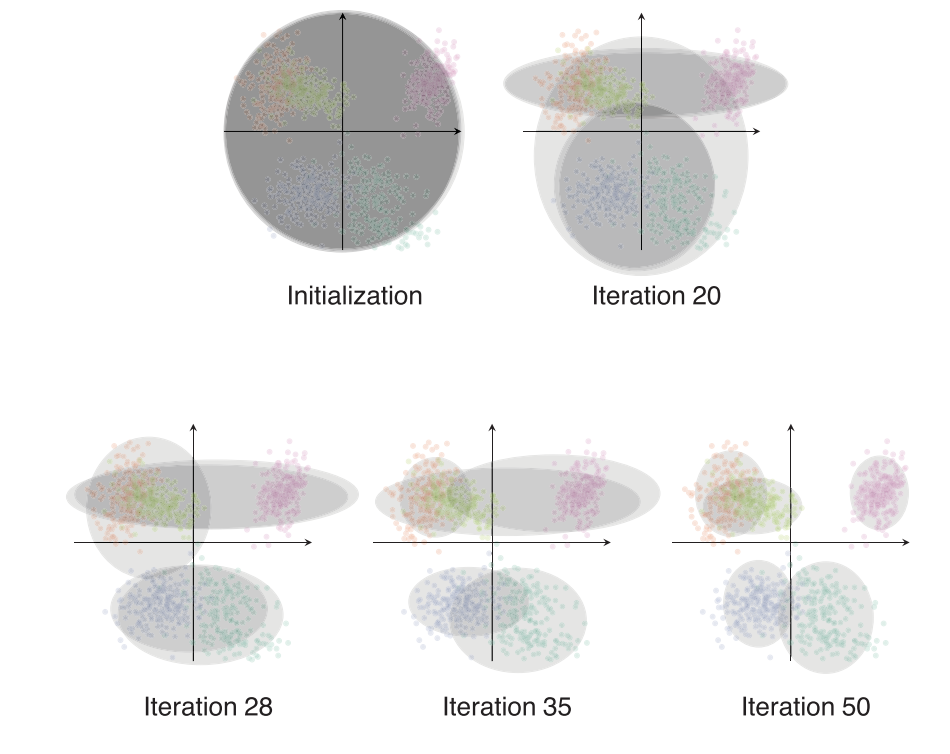
\includegraphics[width=.4\textwidth]{images/GMM}
\end{center}


}

\only<2>{
The joint density, by chain rule, is
\[ p(\+x,\+c,\+\mu) = p(\+\mu) \ds\prod_{i=1}^n p(\+c_i) p(x_i \cond \+c_i, \+\mu) \]
\pause 
And a mean-field variational family is given by 
\[  q(\+c, \+\mu) = \ds\prod_{k=1}^K q(\mu_k) \ds\prod_{i=1}^n q(\+c_i) \]
}

\end{frame}

\begin{frame}{Example: Bayesian Gaussian Mixture Model}
We apply \eqref{eqn:mfcavi_update_2} to determine the coordinate updates for $q_{c_i}$, the variational factors governing cluster assignments.   We take the log of the joint and discard terms that do not depend upon $c_i$ to obtain

\begin{align*}
q(c_{ik}) & \propto \exp \bigg\{ \E_{q_{\mu_k}} \bigg[  \log p(c_i =k) + \log p(x_i \cond c_i=k, \mu) \bigg] \bigg\} \\
& \propto \exp \bigg\{ \E_{q_{\mu_k}} \bigg[ \log \pi_k + x_i \mu_k - \df{1}{2} \mu_k^2 \bigg] \bigg\} \\
& \propto \pi_k \exp \bigg\{ x_i \E_{q_{\mu_k}} [\mu_k] - \df{1}{2}  \E_{q_{\mu_k}} [ \mu_k^2] \bigg\} \\
\end{align*}

The coordinate updates for $q_{\mu_k}$ are derived similarly.  They reveal that $q_{\mu_k}$ are Gaussian, and hence the above expectations are easy to compute. 

\end{frame}

\begin{frame}{Bayesian Gaussian Mixture Model: \\ Updates to mixture component means}
Using the same strategy as when updating cluster assignments $c_i$, we obtain

\begin{align*}
q(\mu_k) & \propto \exp \bigg\{ \E_{-q_{\mu_k}} \bigg[  \log p(\mu_k) + \ds\sum_{i=1}^n \log p(x_i \cond c_i=k, \mu) \bigg] \bigg\} \\
& \propto \exp \bigg\{ -\df{1}{2  \sigma^2} \mu_k^2 +  \ds\sum_{i=1}^{n} \E_{q_c} \bigg[ \+1_{c_i=k}\, \bigg(x_i \mu_k - \df{1}{2} \mu_k^2\bigg) \bigg] \bigg\} \\
& \propto \exp \bigg\{ -\df{1}{2} \bigg(\df{1}{ \sigma^2} + \ds\sum_{i=1}^n q(c_{ik}) \bigg) \mu_k^2 \; +  \;  \bigg( \ds\sum_{i=1}^n q(c_{ik})x_i  \bigg) \mu_k \bigg\} \\
\end{align*}

which is an exponential family distribution with sufficient statistics $(\mu_k, \mu_k^2)$, and hence Gaussian.
\end{frame}

\begin{frame}{Bayesian Gaussian Mixture Model: CAVI Algorithm}

\begin{center}
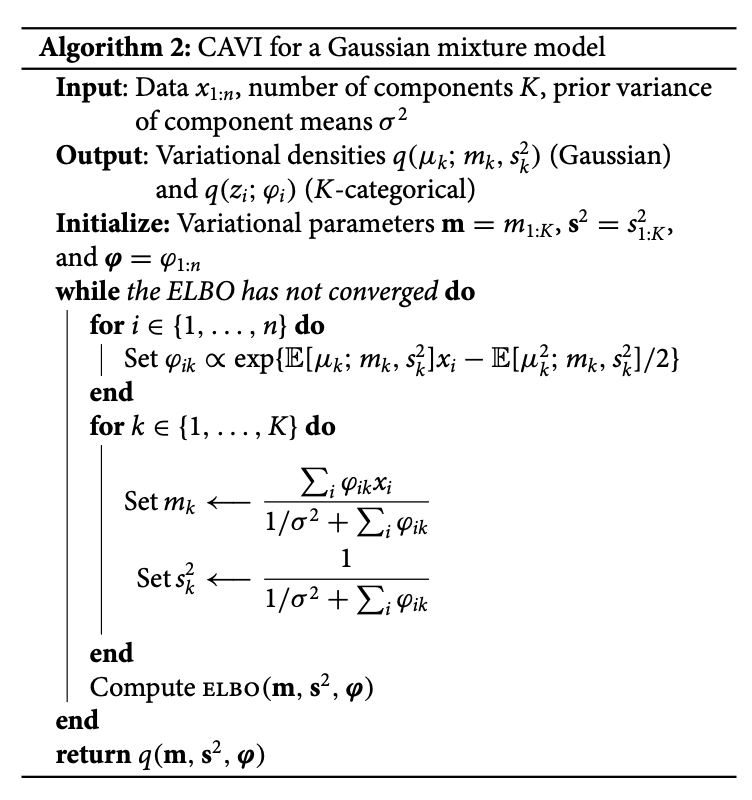
\includegraphics[width=.7\textwidth]{images/GMM_CAVI_algorithm}
\end{center}

\end{frame}


\subsection{A more flexible algorithm: Stochastic Gradient Variational Bayes}

\begin{frame}{The problem with CAVI}
	
\colorbox{red!30}{\textbf{Problem.}} The CAVI updates are:
\begin{align*}
q_k(u_k) \propto \exp \bigg\{ \E_{q_{-k}} \bigg[  \log p(u_k \cond \+u_{-k}, \+x)\bigg] \bigg\}
\end{align*}
What if we can't compute \alert{these} expectations analytically?

\vfill 
\only<2>{
\colorbox{green!30}{\textbf{Big-Picture Idea.}} Let's try to use (stochastic) gradient descent.
}

\end{frame}

\begin{frame}{Older idea}

\only<1->{
\colorbox{blue!30}{\textbf{Recall.}} The objective we're trying to optimize is
 \begin{align*}
\ELBO(q_\phi) & = \explaintermbrace{energy}{\E_{q_\phi} \big[ \log p(\+x, \+z) \big]}  +   \explaintermbrace{entropy}{-\E_{q_\phi}  \big[\log q_\phi(\+z) \big]}
\end{align*}
}


\only<2-3>{
\colorbox{yellow!30}{\textbf{Poll.}}  We'd like to take the gradient $\nabla_\phi \ELBO(q_\phi)$.  Does anybody see a problem?
}

\only<3->{
\colorbox{red!30}{\textbf{Problem.}}  How can we take a gradient the gradient $\nabla_\phi \ELBO(q_\phi)$ if the expectations also depend on $\phi$?
}

\only<4->{
\colorbox{blue!30}{\textbf{An older idea.}} Using the log-derivative trick, we can write
\begin{align*}
\nabla_\phi \E_{q_\phi(\+z)}[f(\+z)] &= 	\E_{q_\phi(\+z)} \bigg[ f(\+z) \nabla_\phi \log q_\phi(\+z) \bigg] \\
&\approx \frac{1}{S} \sum_{s=1}^{S} f(\+z^^s)  \nabla_\phi \log q_\phi(\+z^^s), \qquad \+z^^s \sim q_\phi  
\end{align*}
}

\only<5->{
\colorbox{red!30}{\textbf{Problem.}} This gradient estimator has such high variance that it's unusual.
}

\end{frame}


\begin{frame}{Their idea: Stochastic Gradient Variational Bayes}

\only<1->{
\colorbox{blue!30}{\textbf{Recall.}} The objective we're trying to optimize is
 \begin{align*}
\ELBO(q_\phi) & = \explaintermbrace{energy}{\E_{q_\phi} \big[ \log p(\+x, \+z) \big]}  +   \explaintermbrace{entropy}{-\E_{q_\phi}  \big[\log q_\phi(\+z) \big]}
\end{align*}
}



\only<2->{
\colorbox{green!30}{\textbf{Problem.}}  How can we take a gradient the gradient $\nabla_\phi \ELBO(q_\phi)$ if the expectations also depend on $\phi$?
}

\only<3->{
\colorbox{blue!30}{\textbf{Their idea.}} They use the \alert{``reparametrization trick''}.   They reparameterize the random variable  $\wt{\+z} \sim q_\phi(\+z \mid \+x)$ using a differentiable transformation $g_\phi(\+\epsilon, \+x)$ of an (auxiliary) noise variable $\+\epsilon$:
\[ \wt{\+z} = g_\phi(\+\epsilon, \+x) \qquad \text{with} \qquad \+\epsilon \sim p(\epsilon)\]  
} 

\only<4->{
\colorbox{yellow!30}{\textbf{Who cares?}}
Then they can write \begin{align*}
\E_{q_\phi(\+z \mid \+x_i)}[f(\+z)] &= 	\E_{p(\+\epsilon)} \bigg[ f\big(g_\phi(\+\epsilon, \+x_i)\big)\bigg] \\
&\approx \frac{1}{S} \sum_{s=1}^{S} f\big(g_\phi(\+\epsilon^^s, \+x_i)\big), \qquad \epsilon^^s \sim p(\+\epsilon)
\end{align*}

}


\end{frame}


\section{Good, Bad, Ugly, Beautiful}

\begin{frame}{Good, Bad, Ugly, Beautiful}

\textbf{Guidelines}
\begin{enumerate}
	\item \textit{Good, Bad}: Technical content
	\item \textit{Ugly, Beautiful}: Presentational styles
\end{enumerate}

\vfill 


\textbf{Format}
\begin{enumerate}
	\item Small group discussion
	\item Class discussion 
\end{enumerate}
	
\end{frame}






\end{document}

